\section{Introduction}\label{sec:intro}
The success of a software testing technique is mainly based on the number of faults it discovers in the Software Under Test (SUT). An efficient testing process discovers the maximum number of faults in a minimum possible time. Exhaustive testing, where software is tested against all possible inputs, is mostly not feasible because of the large size of the input domain, limited resources and strict time constraints. Therefore, strategies in automated software testing tools are developed with the aim to select more fault-finding test input from input domain for a given SUT. Producing such targeted test input is difficult because each system has its own requirements and functionality.

Chan et al.~\cite{Chan1996} discovered that there are patterns of failure-causing inputs across the input domain. They divided the patterns into point, block and strip patterns on the basis of their occurrence across the input domain. Chen et al.~\cite{Chen2008} found that the performance of random testing can be increased by slightly altering the technique of test case selection. In adaptive random testing, they found that the performance of random testing increases by up to 50\% when test input is selected evenly across the whole input domain. This was mainly attributed to the better distribution of input which increased the chance of selecting inputs from failure patterns. Similarly Restricted Random Testing \cite{Chan2002}, Feedback directed Random Test Generation \cite{Pacheco2007a}, Mirror Adaptive Random Testing \cite{Chen2003} and Quasi Random Testing \cite{Chen2005} stress the need for test case selection covering the whole input domain to get better results.

In this paper we take the assumption that for a significant number of classes failure domains are contiguous or are very close by. From this assumption, we devised the Dirt Spot Sweeping\footnote{The name refers to the cleaning robots strategy which insists on places where dirt has been found in large amount.} Random (DSSR) strategy  which starts as a random+ strategy --- a random strategy focusing more on boundary values. When a new failure is found, it increases the chances of finding more faults using neighbouring values. As in previous studies~\cite{Oriol2012} we approximate faults with unique failures. Since this strategy is an extension of random testing strategy, it has the full potential to find all unique failures in the program, but additionally we expect it to be faster at finding unique failures, for classes in which failure domains are contiguous, as compared with random (R) and random+ (R+) strategies.

We implemented the DSSR strategy in the random testing tool YETI\footnote{\url{http://www.yetitest.org}}. To evaluate our approach, we tested 30 times each one of the 60 classes of 32 different projects from the Qualitas Corpus\footnote{\url{http://www.qualitascorpus.com}} with each of the three strategies R, R+ and DSSR. We observed that for 53\% of the classes all three strategies find the same unique failures, for remaining 47\% DSSR strategy perform up to 33\% better than random strategy and up to 17\% better than random+ strategy.
We also validated the approach by comparing the significance of these results using t-tests and found out that for 7 classes DSSR was significantly better than both R+ and R, for 8 classes DSSR performed similarly to R+ and significantly better than R, while in 2 cases DSSR performed similarly to R and significantly better than R+. In all other cases, DSSR, R+ and R do not seem to perform significantly differently.
Numerically, the DSSR strategy found 43 more unique failures than R and 12 more unique failures than R+ strategy. 

The rest of this paper is organised as follows: \\ Section~\ref{sec:dssr} describes the DSSR strategy. Section~\ref{sec:imp} presents implementation of the DSSR strategy. Section~\ref{sec:eval} explains the experimental setup. Section~\ref{sec:res} shows results of the experiments. Section~\ref{sec:discussion} discusses the results. Section~\ref{sec:rw} presents related work and Section~\ref{sec:conc}, concludes the study.




%%%%%%%%%%%%%%%%%    DIRT SPOT SWEEPING STRATEGY  %%%%%%%%%%%%%%%

\section{Dirt Spot Sweeping Random Strategy}\label{sec:dssr}
The new software testing technique named, Dirt Spot Sweeping Random (DSSR) strategy combines the random+ strategy with a dirt spot sweeping functionality. It is based on two intuitions. First, boundaries have interesting values and using these values in isolation can provide high impact on test results. Second, faults and unique failures reside in contiguous block and strip pattern. If this is true, DSS increase the performance of the test strategy. Before presenting the details of the DSSR strategy, it is pertinent to review briefly the Random and the Random+ strategy.

\subsection{Random Strategy (R)}
The random strategy is a black-box testing technique in which the SUT is executed using randomly selected test data. Test results obtained are compared to the defined oracle, using SUT specifications in the form of contracts or assertions. In the absence of contracts and assertions the exceptions defined by the programming language are used as test oracles. Because of its black-box testing nature, this strategy is particularly effective in testing softwares where the developers want to keep the source code secret~\cite{Chen2010}. The generation of random test data is comparatively cheap and does not require too much intellectual and computational efforts~\cite{Ciupa2009, Ciupa2008}. It is mainly for this reason that various researchers have recommended random strategy for automated testing tools \cite{Ciupa2008a}. YETI \cite{Oriol2010a, Oriol2010}, AutoTest \cite{Leitner2007, Ciupa2007}, QuickCheck \cite{Claessen2000}, Randoop \cite{Pacheco2007}, JArtege \cite{Oriat2004} are some of the most common automated testing tools based on random strategy.

\indent Efficiency of random testing was made suspicious with the intuitive statement of Myers \cite{Myers2004} who termed random testing as one of the poorest methods for software testing. However, experiments performed by various researchers, \cite{Ciupa2007, Duran1981, Duran1984, Hamlet1994, Ntafos2001} have proved experimentally that random testing is simple to implement, cost effective, efficient and free from human bias as compared to its rival techniques.

Programs tested at random typically fail a large number of times (there are a large number of calls), therefore, it is necessary to cluster failures that likely represent the same fault. The traditional way of doing it is to compare the full stack traces and error types and use this as an equivalence class~\cite{Ciupa2007,Oriol2012} called a unique failure. This way of grouping failures is also used for random+ and DSSR.

\subsection{Random Plus Strategy (R+)}
The random+ strategy~\cite{Leitner2007} is an extension of the random strategy. It uses some special pre-defined values which can be simple boundary values or values that have high tendency of finding faults in the SUT. Boundary values~\cite{Beizer1990} are the values on the start and end of a particular type. For instance, such values for \verb+int+ could be \verb+MAX_INT+, \verb+MAX_INT-1+, \verb+MAX_INT-2+; \verb+MIN_INT+, \verb-MIN_INT+1-, \verb-MIN_INT+2-. Similarly, the tester might also add some other special values that he considers effective in finding faults for the SUT. For example, if a program under test has a loop from -50 to 50 then the tester can add -55 to -45, -5 to 5 and 45 to 55 to the pre-defined list of special values. This static list of interesting values is manually updated before the start of the test and has slightly high priority than selection of random values because of more relevance and high chances of finding faults for the given SUT. These special values have high impact on the results, particularly for detecting problems in specifications~\cite{Ciupa2008}.


\subsection{Dirt Spot Sweeping (DSS)}
Chan et al.~\cite{Chan1996} found that there are patterns of failure-causing inputs across the input domain. Figure \ref{fig:patterns} shows these patterns for two dimensional input domain. They divided these patterns into three types called points, block and strip patterns. The black area (points, block and strip) inside the box show the input which causes the system to fail while white area inside the box represent the genuine input. Boundary of the box (black solid line) surrounds the complete input domain and represents the boundary values. They argue that a strategy has more chances of hitting these fault patterns if test cases far away from each other are selected. Other researchers~\cite{Chan2002, Chen2003, Chen2005}, also tried to generate test cases further away from one another targeting these patterns and achieved better performance. Such increase in performance indicate that faults more often occur contiguous across the input domain. In Dirt Spot Sweeping we propose that if a value reveals fault from the block or strip pattern then for the selection of the next test value, DSS may not look farthest away from the known value and rather pick the closest test value to find another fault from the same region.

\begin{figure}[ht]                                    
\centering
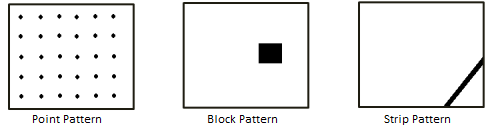
\includegraphics[width= 8cm,height=2.5cm]{DSSR/ART_Patterns.png}
\caption{Failure patterns across input domain~\cite{Chen2008}}
\label{fig:patterns}
\end{figure}

Dirt spot sweeping is the part of DSSR strategy that comes into action when a failure is found in the system. On finding a failure, it immediately adds the value causing the failure and its neighbouring values to the existing list of interesting values. For example, in a program when the \verb+int+ type value of 50 causes a failure in the system then spot sweeping will add values from 47 to 53 to the list of interesting values. If the failure lies in the block or strip pattern, then adding it's neighbouring values will explore other failures present in the block or strip. As against random plus where the list of interesting values remain static, in DSSR strategy the list of interesting values is dynamic and changes during the test execution of each program.

\begin{figure}[ht]
\centering
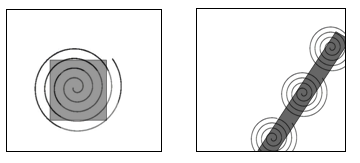
\includegraphics[width=8cm,height=2.2cm]{DSSR/block2.png}
\caption{DSSR covering block and strip pattern}
\label{fig:block2}
\end{figure}

Figure \ref{fig:block2} shows how DSS explores the failures residing in the block and strip patterns of a program. The coverage of block and strip pattern is shown in spiral form because first failure leads to second, second to third and so on till the end. In case the failure is positioned on the point pattern then the added values may not be effective because point pattern is only an arbitrary failure point in the whole input domain.

\subsection{Structure of the Dirt Spot Sweeping Random Strategy}

The DSSR strategy continuously tracks the number of failures during the execution of the test. This tracking is done in a very effective way with zero or minimum overhead to keep the overhead up to bare minimum~\cite{Leitner2009}. The test execution is started by R+ strategy and continues till a failure is found in the SUT after which the program copies the values leading to the failure as well as the surrounding values to the variable list of interesting values. 

\begin{figure}[ht]
\centering
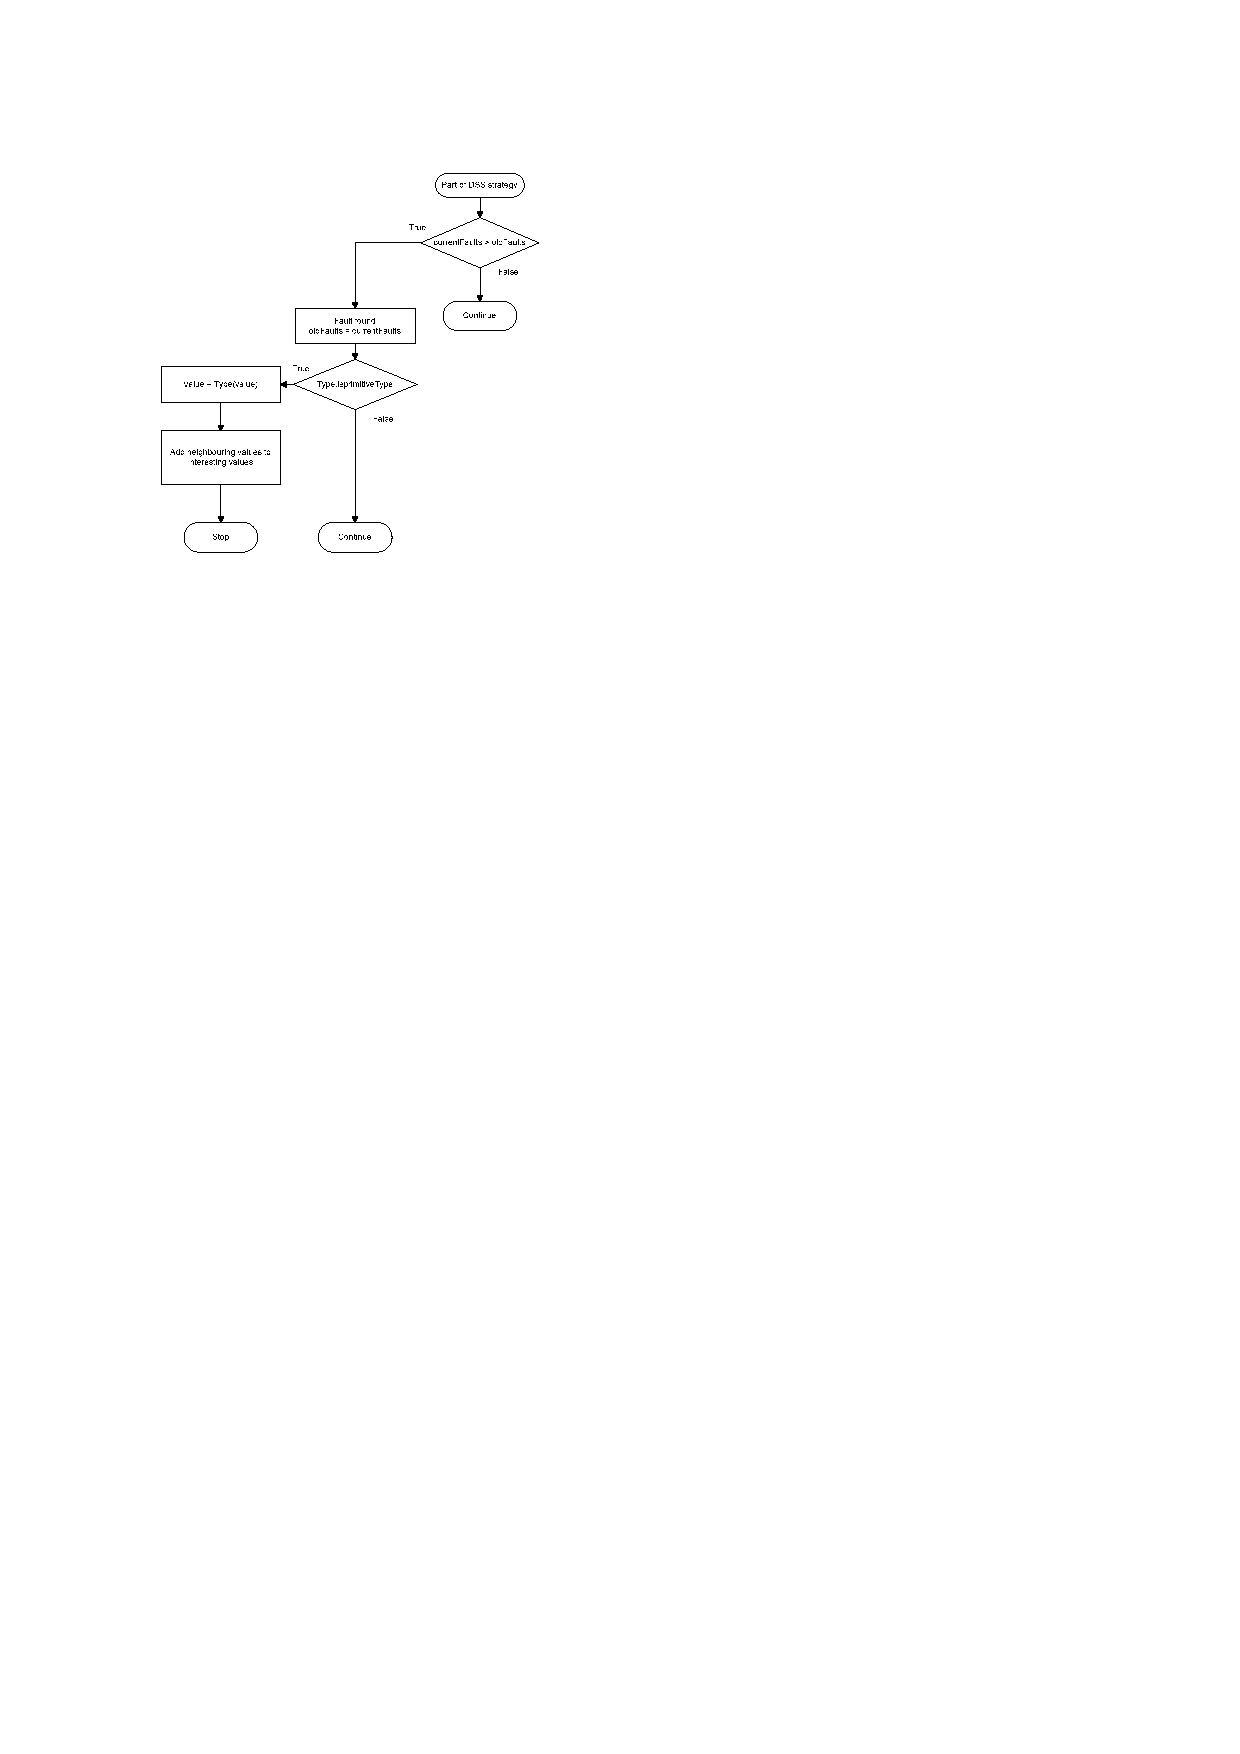
\includegraphics[width=\columnwidth]{DSSR/flowchart1.pdf}
\caption{Working mechanism of DSSR Strategy}
\label{fig:Working_DSSS}
\end{figure}

The flowchart presented in Figure~\ref{fig:Working_DSSS} depicts that, when the failure finding value is of primitive type, the DSSR strategy identifies its type and add values only of that particular type to the list of interesting values. The resultant list of interesting values provide relevant test data for the remaining test session and the generated test cases are more targeted towards finding new failures around the existing failures in the given SUT.

Boundary and other special values that have a high tendency of finding faults in the SUT are added to the list of interesting values by random+ strategy prior to the start of test session where as in DSSR strategy the fault-finding and its surrounding values are added at runtime when a failure is found. 

Table \ref{table:addvalues} presents the values are added to the list of interesting values when a failure is found. In the table the test value is represented by X where X can be int, double, float, long, byte, short, char and String. All values are converted to their respective types before adding them to the list of interesting values.

\begin{table}[ht]
%\scriptsize
\caption{Neighbouring values for primitive types and String} % title of Table
\centering % used for centering table
\begin{tabular}{| l | l |} % centered columns (4 columns)
\hline\hline %inserts double horizontal lines
Type & Values to be added\\ [0.5ex] % inserts table
%heading
\hline % inserts single horizontal line
\multirow{1}{*}{X is int, double, float, } & ~ X,  X+1, X+2, X-1, X-2 \\ % inserting body of the
\multirow{1}{*}{long, byte, short \& char} &  \\ 

\hline
\multirow{8}{*}{X is String} & ~ X\\ % inserting body of the table

& ~ X + ``  "\\ % inserting body of the table
& ~ ``  " + X \\ % inserting body of the table
& ~ X.toUpperCase() \\
& ~ X.toLowerCase() \\
& ~ X.trim() \\
& ~ X.substring(2) \\
& ~ X.substring(1, X.length()-1) \\[1ex]
\hline
\hline %inserts single line
\end{tabular}
\bigskip
\label{table:addvalues} % is used to refer this table in the text
\end{table}





%%%%%%%%%%%%%%%%%%%%%%%%%%%%% EXPLANATION OF DSSR STRATEGY %%%%%%%%%%%%%%%%%%%%%%%%%%


\subsection{Explanation of DSSR strategy on a concrete example}
The DSSR strategy is explained through a simple program seeded with three faults. The first fault is a division by zero exception denoted by 1 while the second and third faults are failing assertion denoted by 2 and 3 in the given program below followed by description of how the strategy perform execution.

\begin{lstlisting}
/** 
* Calculate square of given number 
* and verify results. 
* The code contain 3 faults.
* @author (Mian and Manuel)
*/
public class Math1 {
 public void calc (int num1) {
  // Square num1 and store result. 
  int result1 = num1 * num1;
  int result2 = result1 / num1; // 1
  assert Math.sqrt(result1) == num1; // 2
  assert result1 >= num1; // 3
 } 
}
\end{lstlisting}

In the above code, one primitive variable of type \verb+int+ is used, therefore, the input domain for DSSR strategy is from \verb+-2,147,483,648 to 2,147,483,647+. The strategy further select values (\verb+0, Integer.MIN_VALUE+ \& \verb+Integer.MAX_VALUE+) as interesting values which are prioritised for selection as inputs. 
As the test starts, three faults are quickly discovered by DSSR strategy in the following order.

\indent \textbf{Fault 1:} The strategy select value \verb+0+ for variable \verb+num1+  in the first test case because \verb+0+ is available in the list of interesting values and therefore its priority is higher than other values. This will cause Java to generate division by zero exception (1).

\indent \textbf{Fault 2:} After discovering the first fault, the strategy adds it and its surrounding values to the list of interesting values i.e. \verb+0, 1, 2, 3 and -1, -2, -3+ in this case. In the second test case the strategy may pick \verb+-3+ as a test value which may lead to the second fault where assertion (2) fails because the square root of \verb+9+ is \verb+3+ instead of the input value -3.

\indent \textbf{Fault 3:} After a few tests the strategy may select \\ \verb+Integer.MAX_VALUE+ for variable \verb+num1+  from the list of interesting values leading to discovery of the 3rd fault because int variable \verb+result1+ will not be able to store the square of \\ \verb+Integer.MAX_VALUE+. Instead of the actual square value Java assigns a negative value (Java language rule) to variable result1 that will lead to the violation of the next assertion (3).

The above process explains that including the border, fault-finding and surrounding values to the list of interesting values in DSSR strategy lead to the available faults quickly and in fewer tests as compared to random and random+ strategy. R and R+ takes more number of tests and time to discover the second and third faults because in these strategies the search for new unique failures starts again randomly in spite of the fact that the remaining faults are very close to the first one.


%%%%%%%%%%%%%%%%%    IMPLEMENTATION OF DSSR STRATEGY   %%%%%%%%%%%%


\section{Implementation of the DSSR \\ strategy}\label{sec:imp}

Implementation of the DSSR strategy is made in the YETI open-source automated random testing tool. YETI, coded in Java language, is capable of testing systems developed in procedural, functional and object-oriented languages. Its language-agnostic meta model enables it to test programs written in multiple languages including Java, C\#, JML and .Net. The core features of YETI include easy extensibility for future growth, high speed ( up to one million calls per minute on java code), real time logging, real time GUI support, capability to test programs with multiple strategies and auto generation of test report at the end of test session. For large-scale testing there is a cloud-enabled version of YETI, capable of executing parallel test sessions in Cloud~\cite{Oriol2010}. A number of hitherto faults have successfully been found by YETI in various production softwares~\cite{Oriol2011, Oriol2012}.

YETI can be divided into three decoupled main parts: the core infrastructure, language-specific bindings and strategies. The core infrastructure contains representation for routines, a group of types and a pool of specific type objects. The language specific bindings contain the code to make the call and process the results. The strategies define the procedure of selecting the modules (classes), the routines (methods) and generation of values for instances involved in the routines. By default, YETI uses the random strategy if no particular strategy is defined during test initialisation. It also enables the user to control the probability of using null values and the percentage of newly created objects for each test session. YETI provides an interactive Graphical User Interface (GUI) in which users can see the progress of the current test in real time. In addition to GUI, YETI also provides extensive logs of the test session for more in-depth analysis.

The DSSR strategy is an extension of YetiRandomPlusStrategy, an extended form of the YetiRandomStrategy. The class hierarchy is shown in Figure \ref{fig:hierarchyofDSSR}.

\begin{figure}[h]
\centering
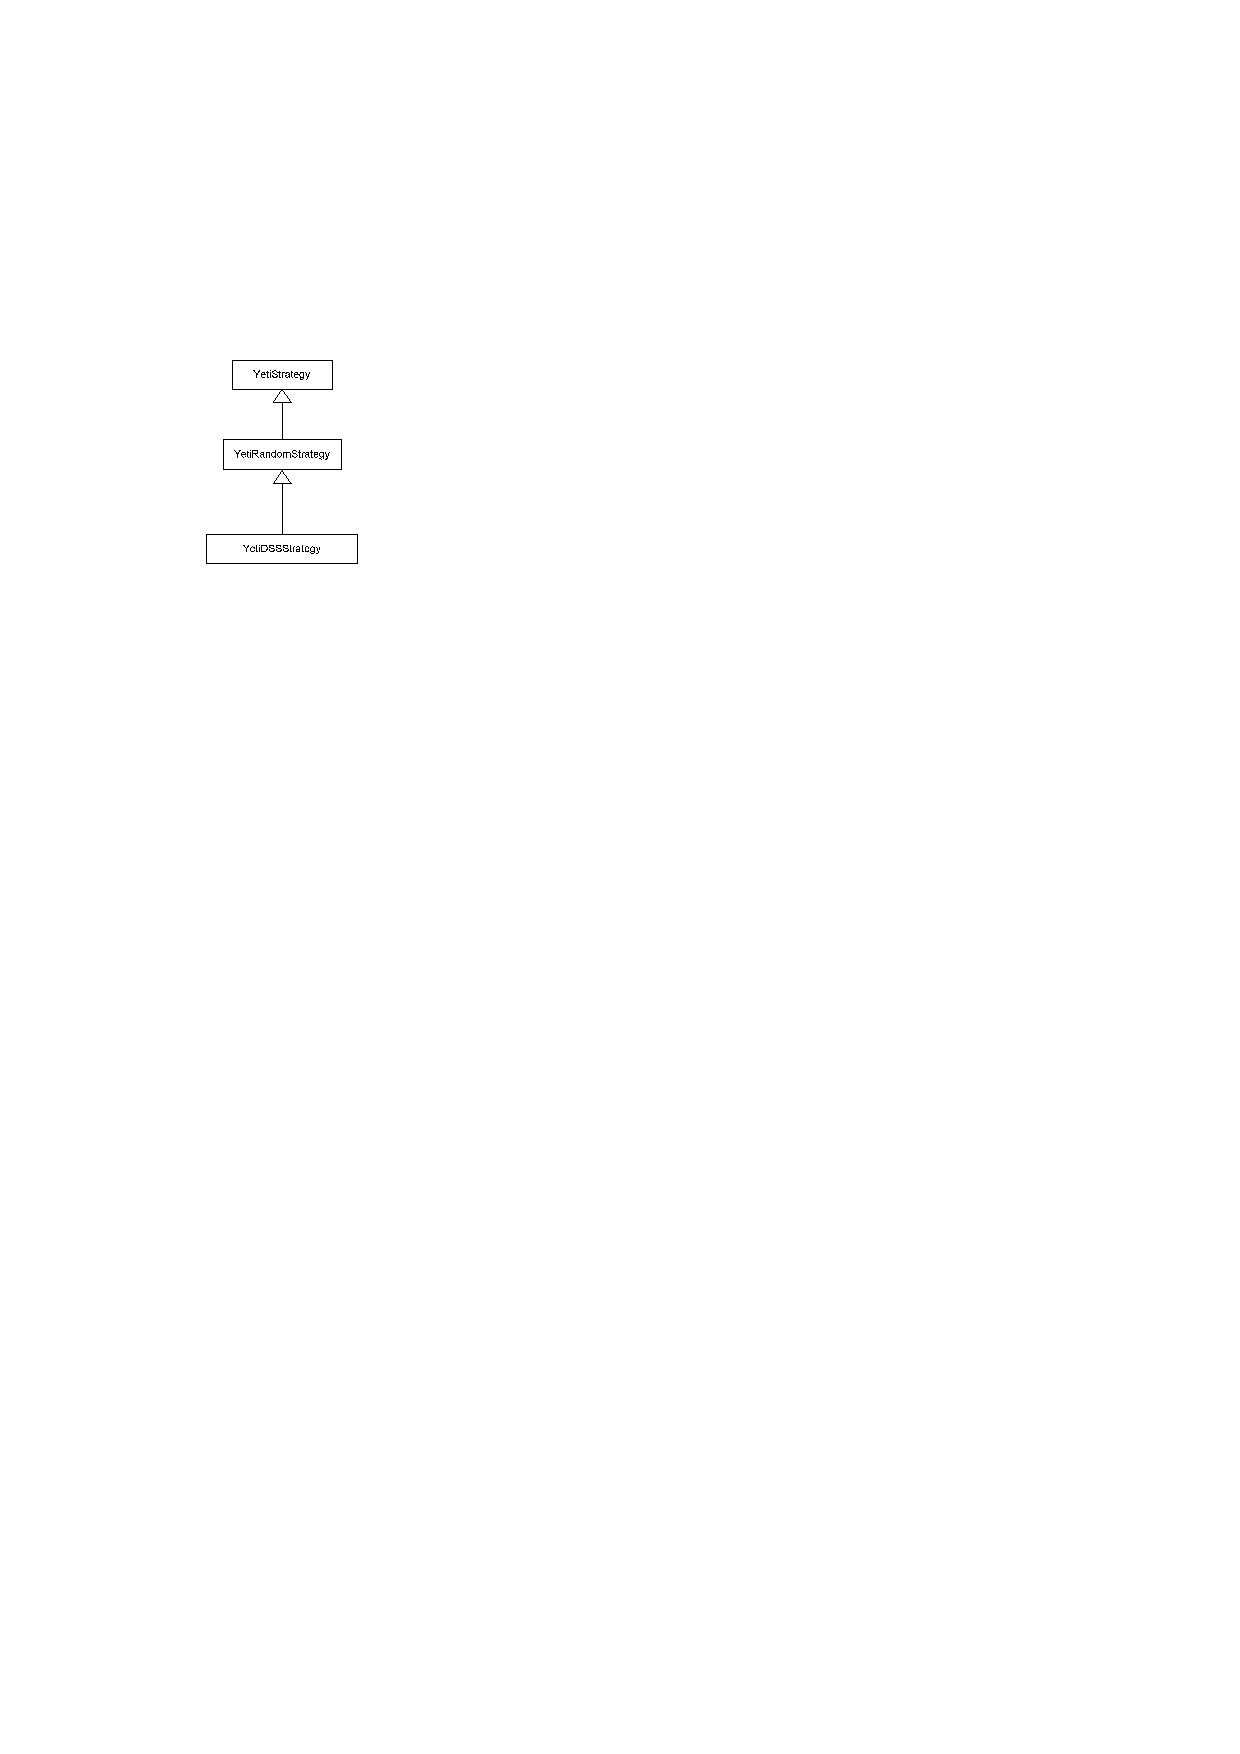
\includegraphics[width=4cm,height=5cm]{DSSR/hierarchy.pdf}
\caption{Class Hierarchy of DSSR in YETI}
\label{fig:hierarchyofDSSR}
\end{figure}





%%%%%%%%%%%%%%%%%    EVALUATION   %%%%%%%%%%%%%%%%%%%%


\section{Evaluation}\label{sec:eval}

The DSSR strategy is experimentally evaluated by comparing its performance with that of random and random+ strategy ~\cite{Leitner2007}. General factors such as system software and hardware, YETI specific factors like percentage of null values, percentage of newly created objects and interesting value injection probability have been kept constant in the experiments.

\subsection{Research questions}
For evaluating the DSSR strategy, the following research questions have been addressed in this study:
\begin{enumerate}
\item Is there an absolute best among R, R+ and DSSR strategies?
\item Are there classes for which any of the three strategies provide better results?
\item Can we pick the best default strategy between R, R+ and DSSR?
\end{enumerate}



\subsection{Experiments}

To evaluate the performance of DSSR we performed extensive testing of programs from the Qualitas Corpus~\cite{Tempero2010a}. The Qualitas Corpus is a curated collection of open source java projects built with the aim of helping empirical research on  software engineering. These projects have been collected in an organised form containing the source and binary forms. Version 20101126, which contains 106 open source java projects is used in the current evaluation. In our experiments we selected 60 random classes from 32 random projects. All the selected classes produced at least one fault and did not time out with maximum testing session of 10 minutes. Every class is tested thirty times by each strategy (R, R+, DSSR). Name, version and size of the projects to which the classes belong are given in table~\ref{table:projects} while test details of the classes is presented in table~\ref{table:Results}. Line of Code (LOC) tested per class and its total is shown in column 3 of table~\ref{table:Results}. 

Every class is evaluated through $10^5$ calls in each test session.\footnote{The total number of tests is thus $60\times 30\times 3 \times 10^5 = 540\times 10^6~tests$.} 
Because of the absence of the contracts and assertions in the code under test, Similar approach as used in previous studies ~\cite{Oriol2012} is followed using undeclared exceptions to compute unique failures.


\begin{table}[h]
\caption{Name and versions of 32 Projects randomly selected from the Qualitas Corpus for the experiments}
\centering
\begin{tabular}{|r|l|r|r|}
\hline
S. No& 	Project Name	& 	Version		&	Size (MB)\\
\hline
1	&	apache-ant	&	1.8.1			&	59\\
2	&	antlr			&	3.2			&	13\\
3	&	aoi			&	2.8.1			&	35\\
4	&	argouml		&	0.30.2		&	112\\
5	&	artofillusion	&	281			&	5.4\\
6	&	aspectj		&	1.6.9			&	109.6\\
7	&	axion		&	1.0-M2		&	13.3\\
8	&	azureus		&	1			&	99.3\\
9	&	castor		&	1.3.1			&	63.2\\
10	&	cayenne		&	3.0.1			&	4.1\\
11	&	cobertura		&	1.9.4.1		&	26.5\\
12	&	colt			&	1.2.0			&	40\\
13	&	emma		&	2.0.5312		&	7.4\\
14	&	freecs		&	1.3.20100406	&	11.4\\
15	&	hibernate		&	3.6.0			&	733\\
16	&	hsqldb		&	2.0.0			&	53.9\\
17	&	itext			&	5.0.3			&	16.2\\
18	&	jasml		&	0.10			&	7.5 \\
19	&	jmoney		&	0.4.4			&	5.3\\
20	&	jruby			&	1.5.2			&	140.7\\
21	&	jsXe			&	04\_beta		&	19.9\\
22	&	quartz		&	1.8.3			&	20.4\\
23	&	sandmark		&	3.4			&	18.8\\
24	&	squirrel-sql	&	3.1.2			&	61.5\\
25	&	tapestry		&	5.1.0.5		&	69.2\\
26	&	tomcat		&	7.0.2			&	24.1\\
27	&	trove			&	2.1.0			&	18.2\\
28	&	velocity		&	1.6.4			&	27.1\\
29	&	weka		&	3.7.2			&	107\\
30	&	xalan		&	2.7.1			&	85.4\\
31	&	xerces		&	2.10.0		&	43.4\\
32	&	xmojo		&	5.0.0			&	15\\
\hline
\end{tabular}
\bigskip
\label{table:projects}
\end{table}



All tests are performed with a 64-bit Mac OS X Lion Version 10.7.4 running on 2 x 2.66 GHz 6-Core Intel Xeon processor with 6 GB (1333 MHz DDR3) of RAM. YETI runs on top of the Java\texttrademark  SE Runtime Environment [version 1.6.0\_35]. The machine took approximately 100 hours to process the experiments.


\subsection{Performance measurement criteria}
Various measures including the E-measure (expected number of failures detected), P-measure (probability of detecting at least one failure) and F-measure (number of test cases used to find the first fault) have been used by researchers to find the effectiveness of the random test strategy. The E-measure and P-measure have been heavily criticised~\cite{Chen2008} and are not considered effective measuring techniques while the F-measure has been often used by various researchers~\cite{Chen1996, Chen2004}. In our initial experiments the F-measure is used to evaluate the efficiency. However it was realised that this is not the right choice. In some experiments a strategy found the first fault quickly than the other but on completion of test session that very strategy found lower number of total faults than the rival strategy. The preference given to a strategy by F-measure because it finds the first fault quickly without giving due consideration to the total number of faults is not fair~\cite{Liu2012}.


  
The literature review revealed that the F-measure is used where testing stops after identification of the first fault and the system is given back to the developers to remove the fault. Currently automated testing tools test the whole system and print all discovered faults in one go therefore, F-measure is not the favourable choice. In our experiments, performance of the strategy is measured by the maximum number of faults detected in SUT by a particular number of test calls \cite{Pacheco2007a, Ciupa2007, Ciupa2008b}. This measurement is effective because it considers the performance of the strategy when all other factors are kept constant.

%%%%%%%%%%%%%%%%%    RESULTS   %%%%%%%%%%%%%%%%%%%%
\begin{figure*}[ht]
\centering
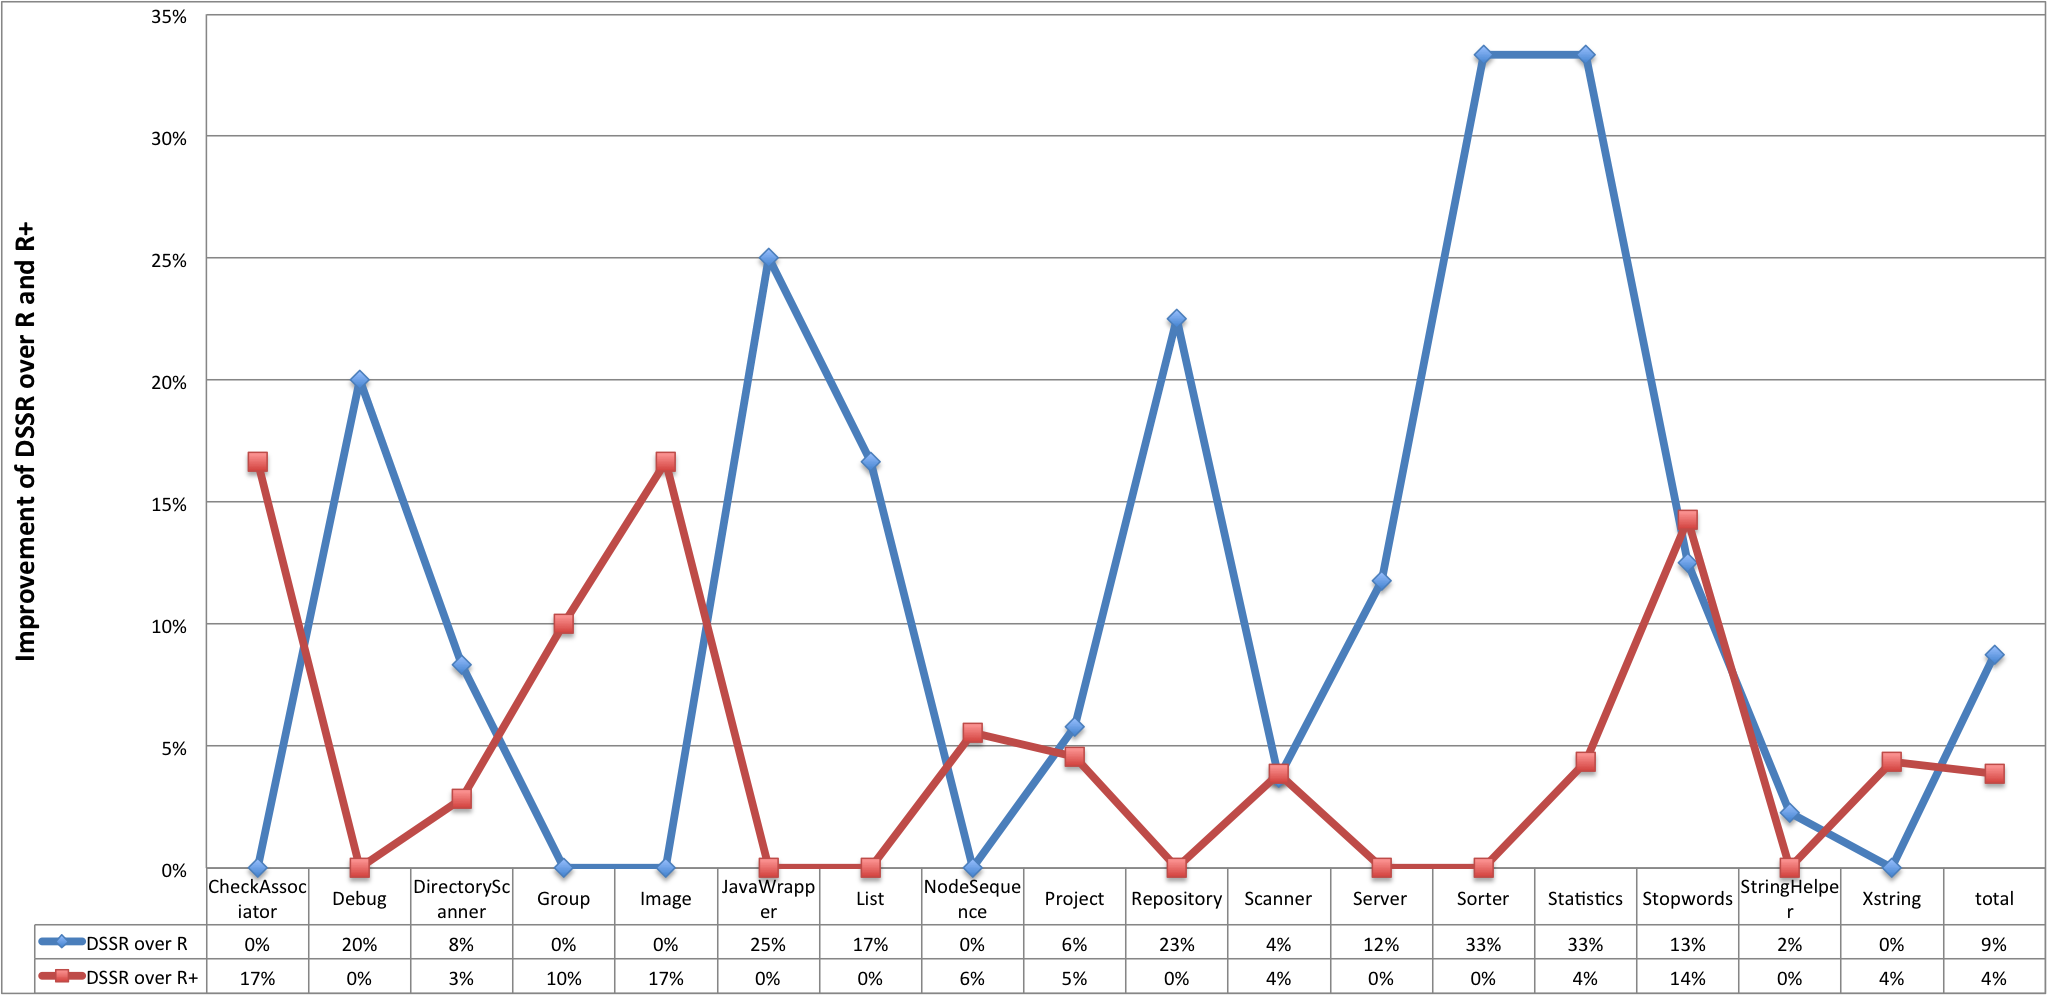
\includegraphics[width=17cm]{DSSR/DssrImprove.png}
\caption{Improvement of DSSR strategy over Random and Random+ strategy.}
\label{fig:LineChart}
\end{figure*}

%%%%%%%%%%%%%%%%%%%%%%%%%%%%%%%%%%%%%%%%%%%%



\begin{table*} [htp!]
  \scriptsize
 \caption{Complete results for R, R+ and DSSR. Results present Serial Number (S.No), Class Name, Line of Code (LOC), mean, maximum number of faults, minimum number of faults and relative standard deviation for each Random (R), Random+ (R+) and Dirt Spot Sweeping Random (DSSR) strategies.}
	%\begin{minipage}[h]{\textwidth}\centering
	\noindent\makebox[\textwidth]{
 	\begin{tabularx}{1 \textwidth}{r l r r r r r r r r r r r r r}
      %\aline
      \multirow{2}{*}{S. No}		& \multirow{2}{*}{Class Name}		& \multirow{2}{*}{LOC}	& \multicolumn{4}{c}{R}							&	\multicolumn{4}{c}{R+}							&	\multicolumn{4}{c}{DSSR}	\\
      %\cline{3-14} 
      						&						&			& Mean 	& Max	& Min 	& 	R-STD				& Mean 	& Max 	& Min 	&	 R-STD 			& Mean 		& Max 		& Min		& R-STD \\

1						& ActionTranslator			&709		& 96		&	96	&	96	& 	0					& 96		& 96 		& 96		& 		0			& 96			& 96			& 96			&	0\\     
2						& AjTypeImpl				&1180		& 80		&	83	&	79	& 	0.02					& 80		& 83 		& 79		& 		0.02			& 80			& 83			& 79			&	0.01\\      
\textbf{3}					& \textbf{Apriori}			&\textbf{292}	& \textbf{3}&	\textbf{4}	&\textbf{3}	& \textbf{0.10}			& \textbf{3}& \textbf{4} 		& \textbf{3}& \textbf{0.13}	& \textbf{3}	& \textbf{4}	& \textbf{3}	&\textbf{0.14}\\      
4						& BitSet					&575		& 9		&	9	&	9	& 	0					& 9		& 9 		& 9		& 		0			& 9			& 9			& 9			&	0\\       
5						& CatalogManager			&538		& 7		&	7	&	7	& 	0					& 7		& 7 		& 7		& 		0			& 7			& 7			& 7			&	0\\    
\textbf{6}					& \textbf{CheckAssociator}	&\textbf{351}	& \textbf{7}	&	\textbf{8}	&	\textbf{2}	& 	\textbf{0.16}					& \textbf{6}		& \textbf{9} 		& \textbf{2}		& 		\textbf{0.18}			& \textbf{7}			& \textbf{9}			& \textbf{6}			&	\textbf{0.73}\\    
\textbf{7}						& \textbf{Debug}					&\textbf{836}		& \textbf{4}		&	\textbf{6}	&	\textbf{4}	& 	\textbf{0.13}					& \textbf{5}		& \textbf{6} 		& \textbf{4}		& 		\textbf{0.12}			& \textbf{5}			& \textbf{8}			& \textbf{4}			&	\textbf{0.19}\\       
\textbf{8}						& \textbf{DirectoryScanner}			&\textbf{1714}		& \textbf{33}		&	\textbf{39}	&	\textbf{20}	& 	\textbf{0.10}					& \textbf{35}		& \textbf{38} 		& \textbf{31}		& 		\textbf{0.05}			& \textbf{36}			& \textbf{39}			& \textbf{32}			&	\textbf{0.04}\\      
9						& DiskIO					&220		& 4		&	4	&	4	& 	0					& 4		& 4 		& 4		& 		0			& 4			& 4			& 4			&	0\\      
10						& DOMParser				&92			& 7		&	7	&	3	& 	0.19					& 7		& 7 		& 3		& 		0.11			& 7			& 7			& 7			&	0\\      
11						& Entities					&328		& 3		&	3	&	3	& 	0					& 3		& 3 		& 3		& 		0			& 3			& 3			& 3			&	0\\      
12						& EntryDecoder			&675		& 8		&	9	&	7	& 	0.10					& 8		& 9 		& 7		& 		0.10			& 8			& 9			& 7			&	0.08\\   
13						& EntryComparator			&163		& 13		&	13	&	13	& 	0					& 13		& 13 		& 13		& 		0			& 13			& 13			& 13			&	0\\      
14						& Entry					&37			& 6		&	6	&	6	& 	0					& 6		& 6 		& 6		& 		0			& 6			& 6			& 6			&	0\\   
15						& Facade					&3301		& 3		&	3	&	3	& 	0					& 3		& 3 		& 3		& 		0			& 3			& 3			& 3			&	0\\   
16						& FileUtil					&83			& 1		&	1	&	1	& 	0					& 1		& 1 		& 1		& 		0			& 1			& 1			& 1			&	0\\      
17						& Font					&184		&12		&	12	&	11	& 	0.03					& 12		& 12 		& 11		& 		0.03			& 12			& 12			& 11			&	0.02\\        
18						& FPGrowth				&435		& 5		&	5	&	5	& 	0					& 5		&  5		& 5		& 		0			& 5			& 5			& 5			&	0	\\       
19						& Generator				&218		& 17		&	17	&	17	& 	0					& 17		& 17 		& 17		& 		0			& 17			& 17			& 17			&	0	\\      
\textbf{20}						& \textbf{Group}					&\textbf{88}			& \textbf{11}		&	\textbf{11}	&	\textbf{10}	& 	\textbf{0.02}					& \textbf{10}		& \textbf{4} 		& \textbf{11}		& 		\textbf{0.15}			& \textbf{11}			& \textbf{11}			& \textbf{11}			&	\textbf{0}	\\      
21						& HttpAuth				&221		& 2		&	2	&	2	& 	0					& 2		& 2 		& 2		& 		0			& 2			& 2			& 2			&	0	\\         
\textbf{22}						& \textbf{Image}					&\textbf{2146}		& \textbf{13}		&	\textbf{17}	&	\textbf{7}	& 	\textbf{0.15}					& \textbf{12}		& \textbf{14} 		& \textbf{4}	& 		\textbf{0.15}			& \textbf{14}			& \textbf{16}			& \textbf{11}			&	\textbf{0.07}\\        
23						& InstrumentTask			&71			& 2		&	2	&	1	& 	0.13					& 2		& 2 		& 1		& 		0.09			& 2			& 2			& 2			&	0	\\    
24						& IntStack					&313		& 4		&	4	&	4	& 	0					& 4		& 4 		& 4		& 		0			& 4			& 4			& 4			&	0	\\      
25						& ItemSet					&234		& 4		&	4	&	4	& 	0					& 4		& 4 		& 4		& 		0			& 4			& 4			& 4			&	0	\\       
26						& Itextpdf					&245		& 8		&	8	&	8	& 	0					& 8		&  8		& 8		& 		0			& 8			& 8			& 8			&	0\\      
\textbf{27}						& \textbf{JavaWrapper}				&\textbf{513}		&\textbf{3}		&	\textbf{2}	&	\textbf{2}	& 	\textbf{0.23}					& \textbf{4}		& \textbf{4} 		& \textbf{3}		& 		\textbf{0.06}			& \textbf{4}			& \textbf{4}			& \textbf{3}			&	\textbf{0.05}\\      
28						& JmxUtilities				&645		& 8		&	8	&	6	& 	0.07					& 8		& 8 		& 7		& 		0.04			& 8			& 8			& 7			&	0.04\\      
\textbf{29}						& \textbf{List}					&\textbf{1718}		& \textbf{5}		&	\textbf{6}	&	\textbf{4}	& 	\textbf{0.11}					& \textbf{6}		& \textbf{6} 		& \textbf{4}		& 		\textbf{0.10}			&\textbf{6}			& \textbf{6}			& \textbf{5}			&	\textbf{0.09}\\      
30						& NameEntry				&172		& 4		&	4	&	4	& 	0					& 4		& 4 		& 4		& 		0			& 4			& 4			& 4			&	0	\\  
\textbf{31}						& \textbf{NodeSequence}			&\textbf{68}			& \textbf{38}		&	\textbf{46}	&	\textbf{30}	& 	\textbf{0.10}					& \textbf{36}		& \textbf{45} 		& \textbf{30}		& 		\textbf{0.12}			& \textbf{38}			& \textbf{45}			& \textbf{30}			&	\textbf{0.08}	\\     
32						& NodeSet				&208		& 28		&	29	&	26	& 	0.03					& 28		& 29 		& 26		& 		0.04			& 28			& 29			& 26			&	0.03	\\  
33						& PersistentBag			&571		& 68		&	68	&	68	& 	0					& 68		&  68		& 68		& 		0			& 68			& 68			& 68			&	0	\\         
34						& PersistentList				&602		& 65		&	65	&	65	& 	0					& 65		&  65		& 65		& 		0			& 65			& 65			& 65			&	0	\\    
35						& PersistentSet				&162		& 36		&	36	&	36	& 	0					& 36		&  36		& 36		& 		0			& 36			& 36			& 36 			&	0	\\        
\textbf{36}						& \textbf{Project}					&\textbf{470}		& \textbf{65}		&	\textbf{71}	&	\textbf{60}	& 	\textbf{0.04}					& \textbf{66}		&  \textbf{78}		& \textbf{62}		& 		\textbf{0.04}			& \textbf{69}			& \textbf{78}			& \textbf{64}			&	\textbf{0.05}	\\        
\textbf{37}						& \textbf{Repository}				&\textbf{63}			& \textbf{31}		&	\textbf{31}	&	\textbf{31}	& 	\textbf{0}					& \textbf{40}		&  \textbf{40}		& \textbf{40}		& 		\textbf{0}			& \textbf{40}			& \textbf{40}			& \textbf{40}			&	\textbf{0}	\\         
38						& Routine					&1069		& 7		&	7	&	7	& 	0					& 7		&  7		& 7		& 		0			& 7			& 7			& 7			&	0	\\
39						& RubyBigDecimal			&1564		& 4 		&	4	&	4	& 	0					& 4		& 4 		& 4		& 		0			& 4			& 4			& 4			&	0\\      
40						& Scanner				&94			& 3		&	5	&	2	& 	0.20					& 3		& 5 		& 2		& 		0.27			& 3			& 5			& 2			&	0.25\\      
\textbf{41}						& \textbf{Scene}					&\textbf{1603}		& \textbf{26}		&	\textbf{27}	&	\textbf{26}	& 	\textbf{0.02}					& \textbf{26}		& \textbf{27} 		& \textbf{26}		& 		\textbf{0.02}			& \textbf{27}			& \textbf{27}			& \textbf{26}			&	\textbf{0.01}\\      
42						& SelectionManager			&431		& 3		&	3	&	3	& 	0					& 3		& 3 		& 3		& 		0			& 3			& 3			& 3			&	0\\      
\textbf{43}						& \textbf{Server}					&\textbf{279}		&\textbf{15}		&	\textbf{21}	&	\textbf{11}	& 	\textbf{0.20}					& \textbf{17}		& \textbf{21} 		& \textbf{12}		& 		\textbf{0.16}			& \textbf{17}			& \textbf{21}			& \textbf{12}			&	\textbf{0.14}\\      
\textbf{44}						& \textbf{Sorter}					&\textbf{47}			& \textbf{2}		&	\textbf{2}	&	\textbf{1}	& 	\textbf{0.09}					& \textbf{3}		& \textbf{3} 		& \textbf{2}		& 		\textbf{0.06}			&\textbf{3}			& \textbf{3}			& \textbf{3}			&	\textbf{0}\\      
45						& Sorting					&762		& 3		&	3	&	3	& 	0					& 3		& 3 		& 3		& 		0			& 3			& 3			& 3			&	0\\      
\textbf{46}						& \textbf{Statistics}				&\textbf{491}		& \textbf{16}		&	\textbf{17}	&	\textbf{12}	&	\textbf{0.08}					& \textbf{23}		& \textbf{25} 		& \textbf{22}		& 		\textbf{0.03}			& \textbf{24}			& \textbf{25}			& \textbf{22}			&	\textbf{0.04}\\      
47						& Status					&32			& 53		&	53	&	53	& 	0					& 53		& 53 		& 53		& 		0			& 53			& 53			& 53			&	0\\      
\textbf{48}						& \textbf{Stopwords}				&\textbf{332}		& \textbf{7}		&	\textbf{8}	&	\textbf{7}	& 	\textbf{0.03}					& \textbf{7}		&  \textbf{8}		& \textbf{6}		& 		\textbf{0.08}			& \textbf{8}			& \textbf{8}			& \textbf{7}			&	\textbf{0.06}\\      
\textbf{49}						& \textbf{StringHelper}				&\textbf{178}		& \textbf{43}	 	& 	\textbf{45}	&	\textbf{40}	& 	\textbf{0.02}					& \textbf{44}		&  \textbf{46}		& \textbf{42}		& 		\textbf{0.02}			& \textbf{44}			& \textbf{45}			& \textbf{42}			&	\textbf{0.02}\\      
50						& StringUtils				&119		& 19 		&	19	&	19	& 	0					& 19		& 19 		& 19		& 		0			& 19			& 19			& 19			&	0\\      
51						& TouchCollector			&222		& 3		&	3	&	3	& 	0					& 3		&  3		& 3		& 		0			& 3			& 3			& 3			&	0\\      
52						& Trie					&460		& 21		&	22	&	21	& 	0.02					& 21		&  22		& 21		& 		0.01			& 21			& 22			& 21			&	0.01\\      
53						& URI					&3970		& 5 		&	5	&	5	& 	0					& 5		&  5		& 5		& 		0			& 5			& 5			& 5			&	0\\      
54						& WebMacro				&311		& 5		&	5	&	5	& 	0					& 5		&  6		& 5		& 		0.14			& 5			& 7			& 5			&	0.28\\      
55						& XMLAttributesImpl			&277		& 8		&	8	&	8	& 	0					& 8		&  8		& 8		& 		0			& 8			& 8			& 8			&	0\\      
56						& XMLChar				&1031		& 13		&	13	&	13	& 	0					& 13		&  13		& 13		& 		0			& 13			& 13			& 13			&	0\\      
57						& XMLEntityManger			&763		& 17		&	18	&	17	& 	0.01					& 17		&  17		& 16		& 		0.01			& 17			& 17			& 17			&	0\\      
58						& XMLEntityScanner			&445		& 12		&	12	&	12	& 	0					& 12		&  12		& 12		& 		0			& 12			& 12			& 12			&	0\\      
59						& XObject					&318		& 19		&	19	&	19	& 	0					& 19		&  19		& 19		& 		0			& 19			& 19			& 19			&	0\\      
\textbf{60}						& \textbf{XString}					&\textbf{546}		& \textbf{23}		&	\textbf{24}	&	\textbf{21}	& 	\textbf{0.04}					& \textbf{23}		&  \textbf{24}		& \textbf{23}		& 		\textbf{0.02}			& \textbf{24}			& \textbf{24}			& \textbf{23}			&	\textbf{0.02}\\      

    						\multicolumn{2}{c}{\textbf{Total}}	&35,785	&1040	&	1075	&    973	&	2.42				& 1061	&1106	&1009	&		2.35		& 1075		& 1118		& 1032		& 	1.82\\
   %\hline
     \end{tabularx} }
 	%\end{minipage}
    \bigskip
    \label{table:Results}
\end{table*}

\section{Results}\label{sec:res}
Results of the experiments including class name, Line of Code (LOC), mean value, maximum and minimum number of unique failures and relative standard deviation for each of the 60 classes tested using R, R+ and DSSR strategy are presented in Table~\ref{table:Results}. Each strategy found an equal number of faults in 31 classes while in the remaining 29 classes the three strategies performed differently from one another. The total of mean values of unique failures in DSSR (1075) is higher than for R (1040) or R+ (1061) strategies. 
%Results given in Table~\ref{table:ttest} can be split into three different categories as shown in Table~\ref{table:categories}. 
DSSR also finds a higher number of maximum unique failures (1118) than both R (1075), and R+ (1106). DSSR strategy finds 43 and 12 more unique faults compared to R and R+ respectively. The minimum number of unique faults found by DSSR (1032) is also higher than for R (973) and R+ (1009) which attributes to higher efficiency of DSSR strategy over R and R+ strategies. 

% How to write relative standard deviation.
% Eventually, the standard deviations are all of the order of magnitude of .1\% for all strategies.

\subsection{Is there an absolute best among R, R+ and DSSR strategies?}
Based on our findings DSSR is at least as good as R and R+ in almost all cases, it is also significantly better than both R and R+ in 12\% of the classes. Figure~\ref{fig:LineChart} presents the average improvements of DSSR strategy over R and R+ strategy over the 17 classes for which there is a significant difference between DSSR and R or R+. The blue line with diamond symbol shows performance of DSSR over R and the red line with square symbols depicts the improvement of DSSR over R+ strategy. The classes where blue line with diamond symbols show the improvement of DSSR over R and red line with square symbols show the improvement of DSSR over R+. 

The improvement of DSSR over R and R+ strategy is calculated by applying the formula (1) and (2) respectively.

\begin{equation} \frac{Averagefaults_{(DSSR)} - Averagefaults_{(R)}}{Averagefaults_{(R)}} * 100  \end{equation}

\begin{equation} \frac{Averagefaults_{(DSSR)} - Averagefaults_{(R+)}}{Averagefaults_{(R+)}}  * 100 \end{equation}

The findings show that DSSR strategy perform up to 33\% better than R and up to 17\% better than R+ strategy. In some cases DSSR perform equally well with R and R+ but in no case DSSR performed lower than R and R+. Based on the results it can be stated that DSSR strategy is a better choice than R and R+ strategy. 



\begin{table*}[htp]
\small
\caption{T-test results of the classes showing different results}
\centering
\begin{tabular}{rlrrrl}
 \multirow{2}{*} {S. No}	& \multirow{2}{*}{Class Name}	&  \multicolumn{3}{c}{T-test Results} & \multirow{2}{*}{Interpretation} \\

								& & 	DSSR, R	& DSSR, R+	&  R, R+ 	& 		\\

1		&	AjTypeImpl		&	1 				& 1 			& 1			& 		\\	
2		&	Apriori			&	\textbf{0.03}	 	& 0.49		& 0.16		&		\\	
3		&	CheckAssociator	&	\textbf{0.04}	 	& \textbf{0.05}	& 0.44		& DSSR better		\\	
4		&	Debug			&	\textbf{0.03}	 	& 0.14		& 0.56		&		\\	
5		&	DirectoryScanner	&	\textbf{0.04}	 	& \textbf{0.01}	& 0.43		& DSSR better		\\
6		&	DomParser		&	\textbf{0.05}	 	& 0.23		& 0.13		&				\\
7		&	EntityDecoder		&	\textbf{0.04}	 	& 0.28		& 0.3			&		\\			
8		&	Font				&	0.18	 			& 0.18		& 1			&		\\
9		&	Group			&	0.33	 			& \textbf{0.03}	& \textbf{0.04}	& DSSR = R > R+	\\
10		&	Image			&	\textbf{0.03}		& \textbf{0.01}	& 0.61		& DSSR better \\		
11		&	InstrumentTask		&	0.16				& 0.33		& 0.57		& \\
12		&	JavaWrapper		&	\textbf{0.001}		& 0.57		& 0.004		& DSSR = R+ > R \\
13		& 	JmxUtilities		&	0.13				& 0.71		& 0.08		&	\\
14		&	List				& 	\textbf{0.01}		&0.25		&\textbf{0}		& DSSR = R+ > R \\
15		&	NodeSequence	&	0.97				&\textbf{0.04}	&\textbf{0.06}	& DSSR = R > R+ \\
16		&	NodeSet			&	\textbf{0.03}		&0.42		&0.26		& 	\\
17		&	Project			&	\textbf{0.001}		&0.57		&\textbf{0.004}	& DSSR better \\		
18		&	Repository		&	\textbf{0}			&1			&\textbf{0}		& DSSR = R+ > R \\
19		&	Scanner			&	1				&\textbf{0.03}	&\textbf{0.01}	& DSSR better \\
20		&	Scene			&	\textbf{0}			&\textbf{0}		& 1			& DSSR better \\
21		&	Server			&	\textbf{0.03}		& 0.88		&\textbf{0.03} 	& DSSR = R+ > R \\
22		&	Sorter			& 	\textbf{0}			& 0.33		&\textbf{0}		& DSSR = R+ > R \\
23		&	Statistics			&	\textbf{0}			& 0.43		&\textbf{0}		& DSSR = R+ > R\\
24		&	Stopwords		&	\textbf{0}			& 0.23		&\textbf{0}		& DSSR = R+ > R \\
25		&	StringHelper		&	\textbf{0.03}		& 0.44		&0.44		& DSSR = R+ > R\\
26		& 	Trie				&	0.1				& 0.33		&0.47		& DSSR better \\
27		&	WebMacro		&	0.33				& 1			&0.16		& \\
28		&	XMLEntityManager	&	0.33				& 0.33		&0.16		& \\
29 		&	XString			&	0.14				&\textbf{0.03}	&0.86		& \\


\end{tabular}
\bigskip
\label{table:ttest}
\end{table*}





\subsection{Are there classes for which any of the three strategies provide better results?}


T-tests applied to the data given in Table~\ref{table:ttest} show that DSSR is significantly better in 7 classes from R and R+ strategy, in 8 classes DSSR performed similarly to R+  but significantly higher than R, and in 2 classes DSSR performed similarly to R but significantly higher than R+. There is no case R and R+ strategy performed significantly better than DSSR strategy. Expressed in percentage: 72\%  of the classes do not show significantly different behaviours whereas in 28\% of hte classes, the DSSR strategy performs significantly better than at least one of R and R+. It is interesting to note that in no single case R and R+ strategies performed better than DSSR strategy. We attribute this to DSSR possessing the qualities of R and R+ whereas containing the spot sweeping feature.


%Results of the 60 classes tested in the study are divided in to 11 different categories as presented in ~\ref{table:categories}. 
\begin{comment}
\begin{table}[h]
\caption{Results of the 60 classes are divided into 11 categories}
\centering
\begin{tabular}{|r|l|r|}
\hline
S. No	& 	Category			& 	Result\\
\hline
1		&	DSSR > R			&	12 \\	
2		&	DSSR > R+		&	10 \\	
3		&	DSSR = R			&	5 \\	
4		&	DSSR = R+		&	7 \\	
5		&	R+ > R 			&	10 \\	
6		&	R+ < R			&	5 \\	
7		&	R+ = R			&	2 \\	
8		&	R > R+			&	4 \\
9		&	DSSR < R			&	0 \\	
10		&	DSSR < R+		&	0 \\
11		&	DSSR = R = R+	&	43 \\			
\hline
\end{tabular}
\bigskip
\label{table:categories}
\end{table}

% pie chart is removed because the length of the paper is exceeding 10 pages and also it don't make much sense i believe.
%\begin{figure}[h]
%\centering
%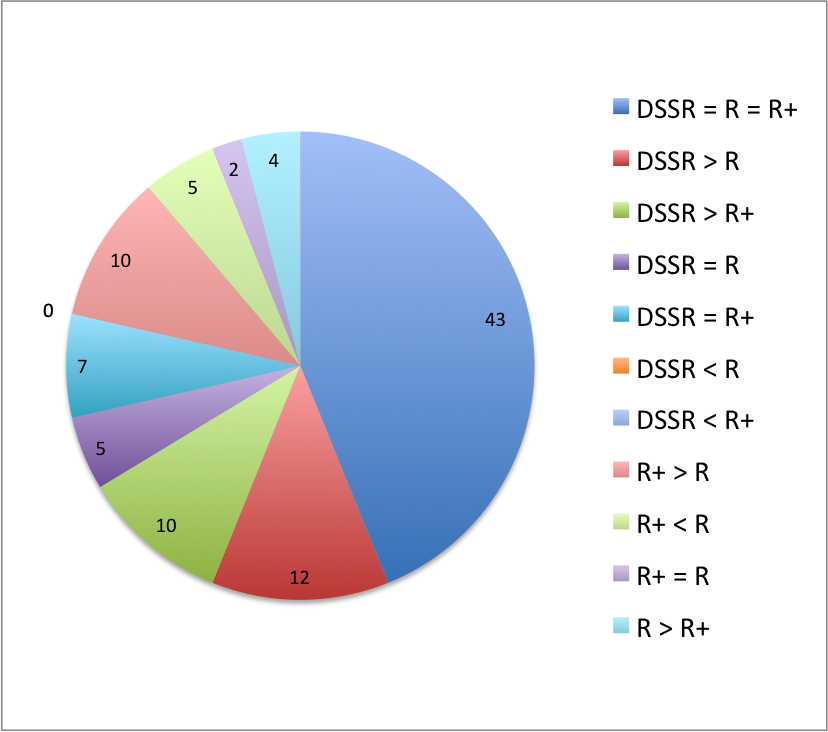
\includegraphics[width=8cm,height=7cm]{pie5.png}
%\caption{Division of result in to categories}
%\label{fig:pie}
%\end{figure}






The first category contain 12 classes where DSSR strategy performs better than R. 
The second category contain 10 classes where DSSR strategy performs better than R+. 
The third category contain 5 classes where DSSR strategy and R performs equally well.
The fourth category contain 7 classes where DSSR and R+ performs equally well. 
The fifth category contain 10 classes where R+ performs better than R.
The sixth category contain 5 classes where R performs better than R+.
The seventh category contain 2 classes where R and R+ performs equally well.
The eighth category contain 4 classes where R performs better than R+.
Category 9 and 10 shows that neither R nor R+ performed better than DSSR strategy.
The last category shows each strategy performing equally well for 43 classes. Expressing in percentage, 72\% classes do not show different behaviours whereas in 28\% of classes, the DSSR strategy performs better than R and R+ strategy. It is interesting to note that in no single case R and R+ strategies performed better than DSSR strategy. This is attributed to the fact that DSSR strategy possess the qualities of R and R+ and has the additional advantage of spot sweeping.

\end{comment}

\subsection{Can we pick the best default strategy between R, R+ and DSSR?}

Analysis of the experimental data reveal that DSSR strategy has an edge over R and R+. This is because of the additional feature of Spot Sweeping in DSSR strategy.

In spite of the better performance of DSSR strategy compared to R and R+ strategies the present study does not provide ample evidence to pick it as the best default strategy because of the overhead induced by this strategy (see next section). Further study might give conclusive evidence. 




%%%%%%%%%%%%%%%%%    DISCUSSION   %%%%%%%%%%%%%%%%%%%%

\section{Discussion}\label{sec:discussion}
In this section we discuss various factors such as the time taken, effect of test duration, number of tests, number of faults in the different strategies and the effect of finding first fault in the DSSR strategy.
\textbf{Time taken to execute an equal number of test cases:}
The DSSR strategy takes slightly more time (up to 5\%) than both pure random and random plus which may be due to maintaining sets of interesting values during the execution. We do not believe that the overhead can be reduced. 

\textbf{Effect of test duration and number of tests on the results:}
All three techniques have the same potential for finding failures. If testing is continued for a long duration then all three strategies will find the same number of unique failures and the results will converge. We suspect however that some of the unique failures will take an extremely long time to be found by using random or random+ only. Further experiments should confirm this point.


\textbf{Effect of number of faults on results:} 
We found that the DSSR strategy performs better when the number of faults is higher in the code. The reason seems to be that when there are more faults, their domains are more connected and DSSR strategy works better. Further studies might use historical data to pick the best strategy.

\textbf{Dependence of DSSR strategy to find the first unique failure early enough:}
During the experiments we noticed that if a unique failure is not found  quickly enough, there is no value added to the list of interesting values and then the test becomes equivalent to random+ testing. This means that better ways of populating failure-inducing values are needed for sufficient leverage to DSSR strategy. As an example, the following piece of code would be unlikely to fail under the current setting:

\begin{lstlisting}
public void test(float value){
 if(value == 34.4445)   10/0;
}
\end{lstlisting}

In this case, we could add constant literals from the SUT to the list of interesting values in a dynamic fashion. These literals can be obtained from the constant pool in the class files of the SUT.

In the example above the value 34.4445 and its surrounding values would  be added to the list of interesting values before the test starts and the DSSR strategy would find the unique failure right away.

\textbf{DSSR strategy and coverage:} Random strategies typically achieve high level of coverage~\cite{Oriol2010}. It might also be interesting to compare R, R+ and DSSR with respect to the achieved coverage or even to use a DSSR variant that adds a new interesting value and its neighbours when a new branch is reached.


\textbf{Threats to validity:} As usual with such empirical studies, the present work might suffer from a non-representative selection of classes.
The selection in the current study is however made through random process and objective criteria, therefore, it seems likely that it would be representative.

The parameters of the study might also have prompted incorrect results. But this is unlikely due to previous results on random testing~\cite{Oriol2012}.



%%%%%%%%%%%%%%%%%    RW   %%%%%%%%%%%%%%%%%%%%

\section{Related Work}\label{sec:rw}

Random testing is a popular technique with simple algorithm but proven to find subtle faults in complex programs and Java libraries~\cite{Pacheco2005, Csallner2004, Claessen2000a}. Its simplicity, ease of implementation and efficiency in generating test cases make it the best choice for test automation~\cite{Hamlet1994}. Some of the well known automated tools based on random strategy includes Jartege~\cite{Oriat2004}, Eclat~\cite{Pacheco2005}, JCrasher~\cite{Csallner2004}, AutoTest \cite{Ciupa2007, Ciupa2008a} and YETI~\cite{Oriol2010, Oriol2012}.

In pursuit of better test results and lower overhead, many variations of random strategy have been proposed~\cite{Chen2010, Chen2005, Chan2002, Chen2004a, Chen2003}. Adaptive random testing (ART), Quasi-random testing (QRT) and Restricted Random testing (RRT) achieved better results by selecting test inputs randomly but evenly spread across the input domain. Mirror ART and ART through dynamic partitioning increased the performance by reducing the overhead of ART. The main reason behind better performance of the strategies is that even spread of test input increases the chance of exploring the fault patterns present in the input domain.

A more recent research study \cite{Yoo2012} stresses on the effectiveness of data regeneration in close vicinity of the existing test data. Their findings showed up to two orders of magnitude more efficient test data generation than the existing techniques. Two major limitations of their study are the requirement of existing test cases to regenerate new test cases, and increased overhead due to ``meta heuristics search'' based on hill climbing algorithm to regenerate new data. In DSSR no pre-existing test cases are required because it utilises the border values from R+ and regenerate the data very cheaply in a dynamic fashion different for each class under test without any prior test data and with comparatively lower overhead. 
  
The random+ (R+) strategy is an extension of the random strategy in which interesting values, beside pure random values, are added to the list of test inputs~\cite{Leitner2007}. These interesting values includes border values which have high tendency of finding faults in the given SUT~\cite{Beizer1990}. Results obtained with R+ strategy show significant improvement over random strategy~\cite{Leitner2007}. DSSR strategy is an extension of R+ strategy which starts testing as R+ until a fault is found then it switches to spot sweeping.

%It is interesting that numerous efforts have been made to discover the fault patterns~\cite{Chen2010, Chen2005, Chan2002, Chen2004a, Chen2003}, etc. but in our knowledge, none has been published on covering/sweeping all the faults lying in a specific pattern once it has been discovered.


A common practice to evaluate performance of an extended strategy is to compare the results obtained by applying the new and existing strategy to identical programs~\cite{Gutjahr1999, Duran1984, Hamlet1990}. Arcuri et al. \cite{Arcuri2012}, stress on the use of random testing as a baseline for comparison with other test strategies. We followed the procedure and evaluated DSSR strategy against R and R+ strategies under identical conditions.

In our experiments we selected projects from the Qualitas Corpus~\cite{Tempero2010} which is a collection of open source java programs maintained for independent empirical research. The projects in Qualitas Corpus are carefully selected that spans across the whole set of java applications~\cite{Oriol2012, Tempero2010a, Tempero2008}.


%%%%%%%%%%%%%%%%%    CONCLUSIONS   %%%%%%%%%%%%%%%%%%%%


\section{Conclusions}\label{sec:conc}
The main goal of the present study was to develop a new random strategy which could find more faults in lower number of test cases. We developed a new strategy named. ``DSSR strategy'' as an extension of R+, based on the assumption that in a significant number of classes, failure domains are contiguous or located closely. The DSS strategy, a strategy which adds neighbouring values of the failure finding value to a list of interesting values, was implemented in the random testing tool YETI to test 60 classes, 30 times each, from Qualitas Corpus with each of the 3 strategies R, R+ and DSSR. The newly developed DSSR strategy uncovers more unique failures than both random and random+ strategies with a 5\% overhead. We found out that for 7 (12\%) classes DSSR was significantly better than both R+ and R, for 8 (13\%) classes DSSR performed similarly to R+ and significantly better than R, while in 2 (3\%) cases DSSR performed similarly to R and significantly better than R+. In all other cases, DSSR, R+ and R do not seem to perform significantly differently. Overall, DSSR yields encouraging results and advocates to develop the technique further for settings in which it is significantly better than both R and R+ strategies.
